% Options for packages loaded elsewhere
\PassOptionsToPackage{unicode}{hyperref}
\PassOptionsToPackage{hyphens}{url}
%
\documentclass[
]{article}
\usepackage{lmodern}
\usepackage{amssymb,amsmath}
\usepackage{ifxetex,ifluatex}
\ifnum 0\ifxetex 1\fi\ifluatex 1\fi=0 % if pdftex
  \usepackage[T1]{fontenc}
  \usepackage[utf8]{inputenc}
  \usepackage{textcomp} % provide euro and other symbols
\else % if luatex or xetex
  \usepackage{unicode-math}
  \defaultfontfeatures{Scale=MatchLowercase}
  \defaultfontfeatures[\rmfamily]{Ligatures=TeX,Scale=1}
\fi
% Use upquote if available, for straight quotes in verbatim environments
\IfFileExists{upquote.sty}{\usepackage{upquote}}{}
\IfFileExists{microtype.sty}{% use microtype if available
  \usepackage[]{microtype}
  \UseMicrotypeSet[protrusion]{basicmath} % disable protrusion for tt fonts
}{}
\makeatletter
\@ifundefined{KOMAClassName}{% if non-KOMA class
  \IfFileExists{parskip.sty}{%
    \usepackage{parskip}
  }{% else
    \setlength{\parindent}{0pt}
    \setlength{\parskip}{6pt plus 2pt minus 1pt}}
}{% if KOMA class
  \KOMAoptions{parskip=half}}
\makeatother
\usepackage{xcolor}
\IfFileExists{xurl.sty}{\usepackage{xurl}}{} % add URL line breaks if available
\IfFileExists{bookmark.sty}{\usepackage{bookmark}}{\usepackage{hyperref}}
\hypersetup{
  pdftitle={real},
  pdfauthor={Joshua},
  hidelinks,
  pdfcreator={LaTeX via pandoc}}
\urlstyle{same} % disable monospaced font for URLs
\usepackage[margin=1in]{geometry}
\usepackage{color}
\usepackage{fancyvrb}
\newcommand{\VerbBar}{|}
\newcommand{\VERB}{\Verb[commandchars=\\\{\}]}
\DefineVerbatimEnvironment{Highlighting}{Verbatim}{commandchars=\\\{\}}
% Add ',fontsize=\small' for more characters per line
\usepackage{framed}
\definecolor{shadecolor}{RGB}{248,248,248}
\newenvironment{Shaded}{\begin{snugshade}}{\end{snugshade}}
\newcommand{\AlertTok}[1]{\textcolor[rgb]{0.94,0.16,0.16}{#1}}
\newcommand{\AnnotationTok}[1]{\textcolor[rgb]{0.56,0.35,0.01}{\textbf{\textit{#1}}}}
\newcommand{\AttributeTok}[1]{\textcolor[rgb]{0.77,0.63,0.00}{#1}}
\newcommand{\BaseNTok}[1]{\textcolor[rgb]{0.00,0.00,0.81}{#1}}
\newcommand{\BuiltInTok}[1]{#1}
\newcommand{\CharTok}[1]{\textcolor[rgb]{0.31,0.60,0.02}{#1}}
\newcommand{\CommentTok}[1]{\textcolor[rgb]{0.56,0.35,0.01}{\textit{#1}}}
\newcommand{\CommentVarTok}[1]{\textcolor[rgb]{0.56,0.35,0.01}{\textbf{\textit{#1}}}}
\newcommand{\ConstantTok}[1]{\textcolor[rgb]{0.00,0.00,0.00}{#1}}
\newcommand{\ControlFlowTok}[1]{\textcolor[rgb]{0.13,0.29,0.53}{\textbf{#1}}}
\newcommand{\DataTypeTok}[1]{\textcolor[rgb]{0.13,0.29,0.53}{#1}}
\newcommand{\DecValTok}[1]{\textcolor[rgb]{0.00,0.00,0.81}{#1}}
\newcommand{\DocumentationTok}[1]{\textcolor[rgb]{0.56,0.35,0.01}{\textbf{\textit{#1}}}}
\newcommand{\ErrorTok}[1]{\textcolor[rgb]{0.64,0.00,0.00}{\textbf{#1}}}
\newcommand{\ExtensionTok}[1]{#1}
\newcommand{\FloatTok}[1]{\textcolor[rgb]{0.00,0.00,0.81}{#1}}
\newcommand{\FunctionTok}[1]{\textcolor[rgb]{0.00,0.00,0.00}{#1}}
\newcommand{\ImportTok}[1]{#1}
\newcommand{\InformationTok}[1]{\textcolor[rgb]{0.56,0.35,0.01}{\textbf{\textit{#1}}}}
\newcommand{\KeywordTok}[1]{\textcolor[rgb]{0.13,0.29,0.53}{\textbf{#1}}}
\newcommand{\NormalTok}[1]{#1}
\newcommand{\OperatorTok}[1]{\textcolor[rgb]{0.81,0.36,0.00}{\textbf{#1}}}
\newcommand{\OtherTok}[1]{\textcolor[rgb]{0.56,0.35,0.01}{#1}}
\newcommand{\PreprocessorTok}[1]{\textcolor[rgb]{0.56,0.35,0.01}{\textit{#1}}}
\newcommand{\RegionMarkerTok}[1]{#1}
\newcommand{\SpecialCharTok}[1]{\textcolor[rgb]{0.00,0.00,0.00}{#1}}
\newcommand{\SpecialStringTok}[1]{\textcolor[rgb]{0.31,0.60,0.02}{#1}}
\newcommand{\StringTok}[1]{\textcolor[rgb]{0.31,0.60,0.02}{#1}}
\newcommand{\VariableTok}[1]{\textcolor[rgb]{0.00,0.00,0.00}{#1}}
\newcommand{\VerbatimStringTok}[1]{\textcolor[rgb]{0.31,0.60,0.02}{#1}}
\newcommand{\WarningTok}[1]{\textcolor[rgb]{0.56,0.35,0.01}{\textbf{\textit{#1}}}}
\usepackage{graphicx,grffile}
\makeatletter
\def\maxwidth{\ifdim\Gin@nat@width>\linewidth\linewidth\else\Gin@nat@width\fi}
\def\maxheight{\ifdim\Gin@nat@height>\textheight\textheight\else\Gin@nat@height\fi}
\makeatother
% Scale images if necessary, so that they will not overflow the page
% margins by default, and it is still possible to overwrite the defaults
% using explicit options in \includegraphics[width, height, ...]{}
\setkeys{Gin}{width=\maxwidth,height=\maxheight,keepaspectratio}
% Set default figure placement to htbp
\makeatletter
\def\fps@figure{htbp}
\makeatother
\setlength{\emergencystretch}{3em} % prevent overfull lines
\providecommand{\tightlist}{%
  \setlength{\itemsep}{0pt}\setlength{\parskip}{0pt}}
\setcounter{secnumdepth}{-\maxdimen} % remove section numbering
\usepackage{booktabs}
\usepackage{longtable}
\usepackage{array}
\usepackage{multirow}
\usepackage{wrapfig}
\usepackage{float}
\usepackage{colortbl}
\usepackage{pdflscape}
\usepackage{tabu}
\usepackage{threeparttable}
\usepackage{threeparttablex}
\usepackage[normalem]{ulem}
\usepackage{makecell}
\usepackage{xcolor}

\title{real}
\author{Joshua}
\date{}

\begin{document}
\maketitle

\begin{Shaded}
\begin{Highlighting}[]
\KeywordTok{rm}\NormalTok{(}\DataTypeTok{list=}\KeywordTok{ls}\NormalTok{())}
\KeywordTok{library}\NormalTok{(}\StringTok{'knitr'}\NormalTok{)}
\end{Highlighting}
\end{Shaded}

\begin{verbatim}
## Warning: package 'knitr' was built under R version 3.5.2
\end{verbatim}

\begin{Shaded}
\begin{Highlighting}[]
\KeywordTok{library}\NormalTok{(}\StringTok{'kableExtra'}\NormalTok{)}
\end{Highlighting}
\end{Shaded}

\begin{verbatim}
## Warning: package 'kableExtra' was built under R version 3.5.2
\end{verbatim}

\begin{Shaded}
\begin{Highlighting}[]
\KeywordTok{library}\NormalTok{(}\StringTok{'forecast'}\NormalTok{)}
\end{Highlighting}
\end{Shaded}

\begin{verbatim}
## Warning: package 'forecast' was built under R version 3.5.2
\end{verbatim}

\begin{Shaded}
\begin{Highlighting}[]
\KeywordTok{library}\NormalTok{(}\StringTok{'smooth'}\NormalTok{)}
\end{Highlighting}
\end{Shaded}

\begin{verbatim}
## Warning: package 'smooth' was built under R version 3.5.2
\end{verbatim}

\begin{verbatim}
## Loading required package: greybox
\end{verbatim}

\begin{verbatim}
## Warning: package 'greybox' was built under R version 3.5.2
\end{verbatim}

\begin{verbatim}
## Package "greybox", v0.5.8 loaded.
\end{verbatim}

\begin{verbatim}
## This is package "smooth", v2.5.5
\end{verbatim}

\begin{Shaded}
\begin{Highlighting}[]
\KeywordTok{library}\NormalTok{(}\StringTok{'beanplot'}\NormalTok{)}
\KeywordTok{library}\NormalTok{(}\StringTok{'pastecs'}\NormalTok{)}
\KeywordTok{library}\NormalTok{(}\StringTok{'scales'}\NormalTok{)}
\KeywordTok{library}\NormalTok{(}\StringTok{'rbenchmark'}\NormalTok{)}
\KeywordTok{library}\NormalTok{(}\StringTok{'ggplot2'}\NormalTok{)}
\KeywordTok{library}\NormalTok{(}\StringTok{'readxl'}\NormalTok{)}
\end{Highlighting}
\end{Shaded}

\begin{verbatim}
## Warning: package 'readxl' was built under R version 3.5.2
\end{verbatim}

\begin{Shaded}
\begin{Highlighting}[]
\NormalTok{source<-}\KeywordTok{read_excel}\NormalTok{(}\StringTok{'Covid.xlsx'}\NormalTok{,}\DecValTok{2}\NormalTok{,}\DataTypeTok{range =} \KeywordTok{cell_rows}\NormalTok{(}\DecValTok{151}\NormalTok{),}\DataTypeTok{col_names =} \OtherTok{FALSE}\NormalTok{)}
\end{Highlighting}
\end{Shaded}

\begin{verbatim}
## New names:
## * `` -> ...1
## * `` -> ...2
## * `` -> ...3
## * `` -> ...4
## * `` -> ...5
## * ... and 181 more problems
\end{verbatim}

\begin{Shaded}
\begin{Highlighting}[]
\NormalTok{time_series<-}\KeywordTok{ts}\NormalTok{(}\KeywordTok{as.numeric}\NormalTok{(source[}\DecValTok{4}\OperatorTok{:}\DecValTok{183}\NormalTok{]),}\DataTypeTok{frequency =} \DecValTok{7}\NormalTok{, }\DataTypeTok{start =} \KeywordTok{c}\NormalTok{(}\DecValTok{1}\NormalTok{, }\DecValTok{5}\NormalTok{))}
\NormalTok{time_series<-}\KeywordTok{tsclean}\NormalTok{(time_series)}
\NormalTok{horizon<-}\DecValTok{100}
\NormalTok{n<-}\DecValTok{80}
\end{Highlighting}
\end{Shaded}

\begin{Shaded}
\begin{Highlighting}[]
\NormalTok{ts_plot_season <-}\StringTok{ }\ControlFlowTok{function}\NormalTok{(}\DataTypeTok{x =}\NormalTok{ x) \{}
\NormalTok{season <-}\StringTok{ }\KeywordTok{cycle}\NormalTok{(x)}
\NormalTok{season.factor <-}\StringTok{ }\KeywordTok{factor}\NormalTok{(season)}
\KeywordTok{ggplot}\NormalTok{() }\OperatorTok{+}\StringTok{ }
\StringTok{  }\KeywordTok{geom_boxplot}\NormalTok{(}\DataTypeTok{mapping =} \KeywordTok{aes}\NormalTok{(}\DataTypeTok{x =}\NormalTok{ season.factor,}
                             \DataTypeTok{y =}\NormalTok{ x)) }\OperatorTok{+}
\StringTok{  }\KeywordTok{labs}\NormalTok{(}\DataTypeTok{x =} \StringTok{""}\NormalTok{, }\DataTypeTok{y =}  \StringTok{"Bed Occupied"}\NormalTok{) }\OperatorTok{+}
\StringTok{  }\KeywordTok{scale_x_discrete}\NormalTok{(}\DataTypeTok{labels=}\KeywordTok{c}\NormalTok{(}\StringTok{"1"}\NormalTok{ =}\StringTok{ "Sun"}\NormalTok{, }\StringTok{"2"}\NormalTok{ =}\StringTok{ "Mon"}\NormalTok{, }\StringTok{"3"}\NormalTok{ =}\StringTok{ "Tue"}\NormalTok{, }\StringTok{"4"}\NormalTok{ =}\StringTok{ "Wed"}\NormalTok{, }\StringTok{"5"}\NormalTok{ =}\StringTok{ "Thu"}\NormalTok{, }\StringTok{"6"}\NormalTok{ =}\StringTok{ "Fri"}\NormalTok{, }\StringTok{"7"}\NormalTok{ =}\StringTok{ "Sat"}\NormalTok{)) }\OperatorTok{+}
\StringTok{  }\KeywordTok{theme_bw}\NormalTok{()}
\NormalTok{\}}

\NormalTok{data <-}\StringTok{ }\KeywordTok{data.frame}\NormalTok{(}
  \DataTypeTok{day =} \KeywordTok{as.Date}\NormalTok{(}\StringTok{"2020-04-02"}\NormalTok{) }\OperatorTok{+}\StringTok{ }\DecValTok{0}\OperatorTok{:}\DecValTok{179}\NormalTok{,}
  \DataTypeTok{value =} \KeywordTok{as.numeric}\NormalTok{(time_series)}
\NormalTok{)}
\NormalTok{plot <-}\StringTok{ }\KeywordTok{ggplot}\NormalTok{(data, }\KeywordTok{aes}\NormalTok{(}\DataTypeTok{x=}\NormalTok{day, }\DataTypeTok{y=}\NormalTok{value)) }\OperatorTok{+}
\StringTok{  }\KeywordTok{geom_line}\NormalTok{(}\DataTypeTok{size =} \FloatTok{0.7}\NormalTok{) }\OperatorTok{+}\StringTok{ }
\StringTok{  }\KeywordTok{xlab}\NormalTok{(}\StringTok{""}\NormalTok{)}
\NormalTok{plot }\OperatorTok{+}\StringTok{ }\KeywordTok{labs}\NormalTok{(}\DataTypeTok{x =} \StringTok{""}\NormalTok{, }\DataTypeTok{y =}  \StringTok{"Bed Occupied"}\NormalTok{) }\OperatorTok{+}\StringTok{ }\KeywordTok{theme_bw}\NormalTok{()}
\end{Highlighting}
\end{Shaded}

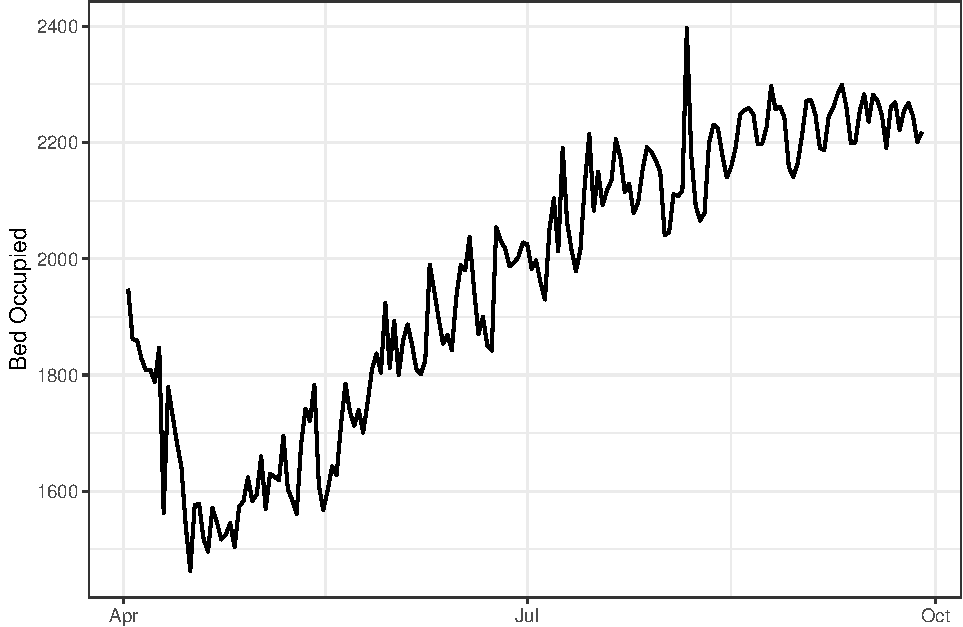
\includegraphics{Real_files/figure-latex/plot-1.pdf}

\begin{Shaded}
\begin{Highlighting}[]
\KeywordTok{ts_plot_season}\NormalTok{(time_series)}
\end{Highlighting}
\end{Shaded}

\begin{verbatim}
## Don't know how to automatically pick scale for object of type ts. Defaulting to continuous.
\end{verbatim}

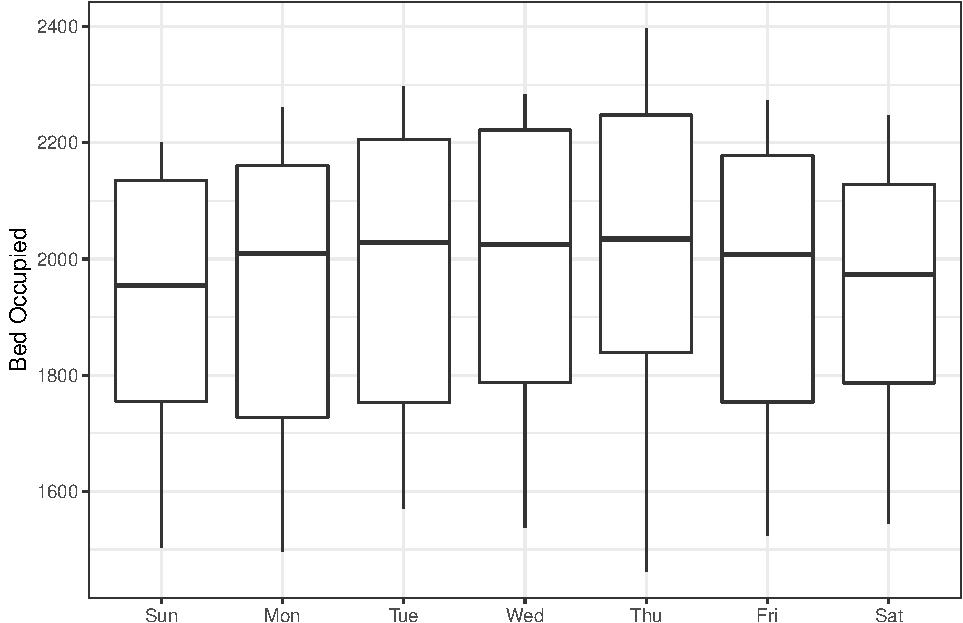
\includegraphics{Real_files/figure-latex/plot-2.pdf}

\begin{Shaded}
\begin{Highlighting}[]
\NormalTok{ts_acf<-}\KeywordTok{Acf}\NormalTok{(time_series,}\DataTypeTok{plot =} \OtherTok{FALSE}\NormalTok{)}
\NormalTok{ts_pacf<-}\KeywordTok{Pacf}\NormalTok{(time_series,}\DataTypeTok{plot =} \OtherTok{FALSE}\NormalTok{)}
\KeywordTok{plot}\NormalTok{(ts_acf, }\DataTypeTok{main =} \StringTok{"Bed Occupied Time Series ACF"}\NormalTok{)}
\end{Highlighting}
\end{Shaded}

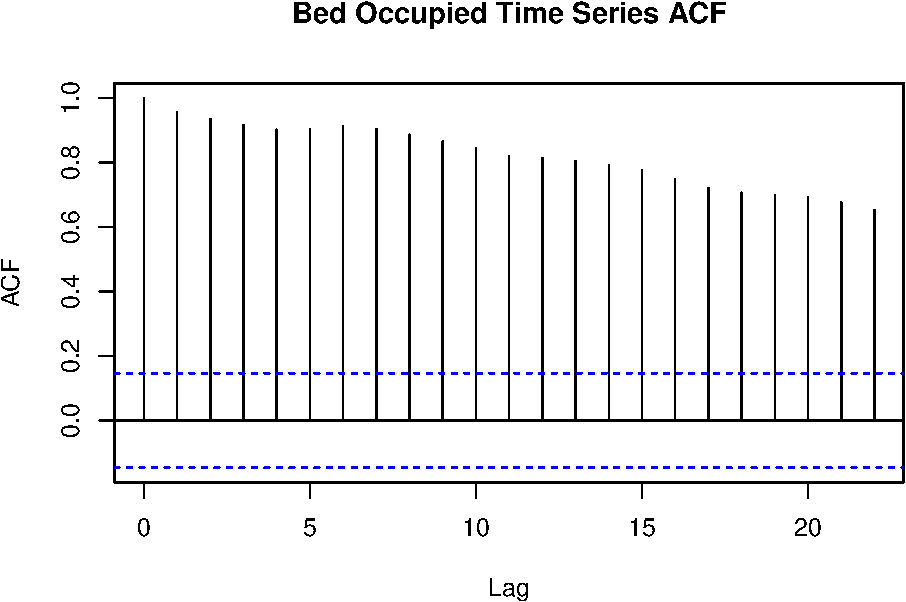
\includegraphics{Real_files/figure-latex/acf-1.pdf}

\begin{Shaded}
\begin{Highlighting}[]
\KeywordTok{plot}\NormalTok{(ts_pacf, }\DataTypeTok{main =} \StringTok{"Bed Occupied Time Series PACF"}\NormalTok{)}
\end{Highlighting}
\end{Shaded}

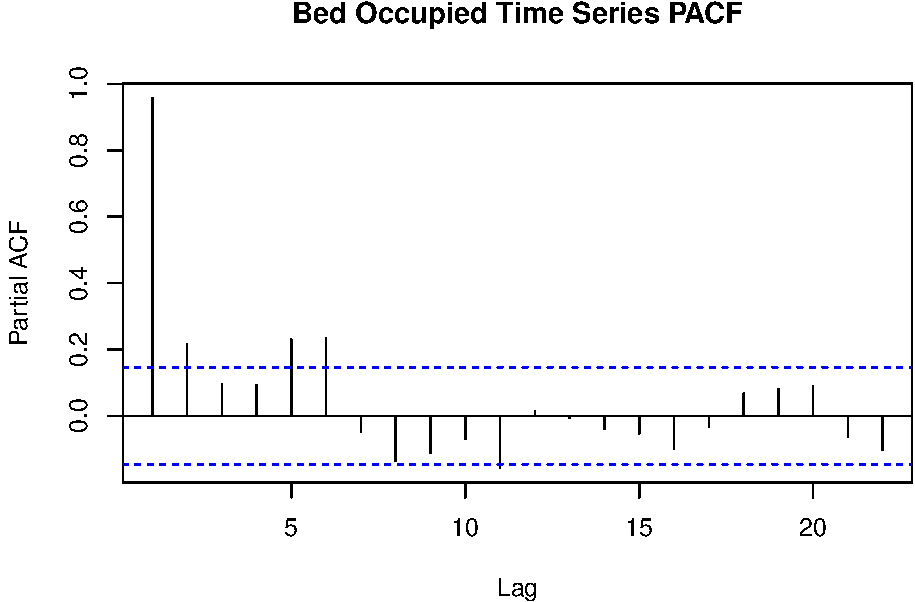
\includegraphics{Real_files/figure-latex/acf-2.pdf}

\begin{Shaded}
\begin{Highlighting}[]
\NormalTok{cost_function<-}\ControlFlowTok{function}\NormalTok{(order,demand)\{}
\NormalTok{  u<-}\KeywordTok{runif}\NormalTok{(}\DecValTok{100}\NormalTok{,}\DecValTok{0}\NormalTok{,}\DecValTok{15}\NormalTok{)}
\NormalTok{  salvage<-}\KeywordTok{mean}\NormalTok{((}\KeywordTok{rep}\NormalTok{((order}\OperatorTok{-}\NormalTok{demand),}\DecValTok{100}\NormalTok{)}\OperatorTok{>=}\NormalTok{u)}\OperatorTok{*}\NormalTok{u}\OperatorTok{+}\NormalTok{(}\KeywordTok{rep}\NormalTok{((order}\OperatorTok{-}\NormalTok{demand),}\DecValTok{100}\NormalTok{)}\OperatorTok{<}\NormalTok{u)}\OperatorTok{*}\KeywordTok{rep}\NormalTok{((order}\OperatorTok{-}\NormalTok{demand),}\DecValTok{100}\NormalTok{))}
\NormalTok{  over<-}\DecValTok{10}\OperatorTok{*}\NormalTok{(order}\OperatorTok{-}\NormalTok{demand)}\OperatorTok{-}\DecValTok{4}\OperatorTok{*}\NormalTok{salvage}
\NormalTok{  under<-(demand}\OperatorTok{-}\NormalTok{order)}\OperatorTok{^}\DecValTok{2}
\NormalTok{  cost<-(order}\OperatorTok{>=}\NormalTok{demand)}\OperatorTok{*}\NormalTok{over}\OperatorTok{+}\NormalTok{(order}\OperatorTok{<}\NormalTok{demand)}\OperatorTok{*}\NormalTok{under}
  \KeywordTok{return}\NormalTok{(cost)}
\NormalTok{\}}
\end{Highlighting}
\end{Shaded}

\begin{Shaded}
\begin{Highlighting}[]
\NormalTok{art_demand<-}\KeywordTok{rnorm}\NormalTok{(}\DecValTok{10000}\NormalTok{,}\DecValTok{700}\NormalTok{,}\DecValTok{50}\NormalTok{)}
\NormalTok{mini_function<-}\ControlFlowTok{function}\NormalTok{(par,list_demand)\{}
\NormalTok{  record<-}\KeywordTok{c}\NormalTok{()}
  \ControlFlowTok{for}\NormalTok{ (i }\ControlFlowTok{in}\NormalTok{ list_demand) \{}
\NormalTok{    co<-}\KeywordTok{cost_function}\NormalTok{(par,i)}
\NormalTok{    record<-}\KeywordTok{c}\NormalTok{(record,co)}
\NormalTok{  \}}
  \KeywordTok{return}\NormalTok{(}\KeywordTok{mean}\NormalTok{(record))}
\NormalTok{\}}
\NormalTok{quan<-}\KeywordTok{mean}\NormalTok{(}\KeywordTok{optim}\NormalTok{(}\DataTypeTok{par =} \DecValTok{700}\NormalTok{, }\DataTypeTok{fn =}\NormalTok{ mini_function,}\DataTypeTok{method =} \StringTok{'L-BFGS-B'}\NormalTok{, }\DataTypeTok{list_demand =}\NormalTok{ art_demand)}\OperatorTok{$}\NormalTok{par}\OperatorTok{>}\NormalTok{art_demand)}
\end{Highlighting}
\end{Shaded}

\begin{Shaded}
\begin{Highlighting}[]
\NormalTok{mini_cost_}\DecValTok{1}\NormalTok{<-}\ControlFlowTok{function}\NormalTok{(data,par)\{}
\NormalTok{  order<-par[}\DecValTok{1}\NormalTok{]}\OperatorTok{+}\NormalTok{par[}\DecValTok{2}\NormalTok{]}\OperatorTok{*}\NormalTok{data[,}\DecValTok{2}\NormalTok{]}
\NormalTok{  total_cost<-}\KeywordTok{sum}\NormalTok{(}\KeywordTok{apply}\NormalTok{(}\KeywordTok{cbind}\NormalTok{(order,data[,}\DecValTok{1}\NormalTok{]),}\DecValTok{1}\NormalTok{,}\ControlFlowTok{function}\NormalTok{(x) }\KeywordTok{cost_function}\NormalTok{(x[}\DecValTok{1}\NormalTok{],x[}\DecValTok{2}\NormalTok{])))}
  \KeywordTok{return}\NormalTok{(total_cost)}
\NormalTok{\}}

\NormalTok{dj_record_}\DecValTok{1}\NormalTok{<-}\KeywordTok{c}\NormalTok{()}
\NormalTok{imeo_record_}\DecValTok{1}\NormalTok{<-}\KeywordTok{c}\NormalTok{()}
\ControlFlowTok{for}\NormalTok{ (i }\ControlFlowTok{in} \DecValTok{1}\OperatorTok{:}\NormalTok{n)\{}
\NormalTok{  train<-}\KeywordTok{ts}\NormalTok{(time_series[i}\OperatorTok{:}\NormalTok{(horizon}\OperatorTok{+}\NormalTok{i}\DecValTok{-1}\NormalTok{)]}\OperatorTok{/}\DecValTok{3}\NormalTok{,}\DataTypeTok{frequency =} \DecValTok{7}\NormalTok{)}
\NormalTok{  L1_train=}\KeywordTok{lag}\NormalTok{(train,}\OperatorTok{-}\DecValTok{1}\NormalTok{)}
\NormalTok{  set_train=}\KeywordTok{cbind}\NormalTok{(train,L1_train)}
  \KeywordTok{colnames}\NormalTok{(set_train)<-}\KeywordTok{c}\NormalTok{(}\StringTok{'train'}\NormalTok{,}\StringTok{'L1'}\NormalTok{)}
\NormalTok{  set_train=}\KeywordTok{ts}\NormalTok{(set_train[}\DecValTok{8}\OperatorTok{:}\NormalTok{horizon,])}
\NormalTok{  dj_fit<-}\KeywordTok{ssarima}\NormalTok{(train,}\DataTypeTok{frequency=}\DecValTok{7}\NormalTok{,}\DataTypeTok{orders=}\KeywordTok{list}\NormalTok{(}\DataTypeTok{ar=}\KeywordTok{c}\NormalTok{(}\DecValTok{1}\NormalTok{,}\DecValTok{0}\NormalTok{)),}\DataTypeTok{lags =}\KeywordTok{c}\NormalTok{(}\DecValTok{1}\NormalTok{,}\DecValTok{7}\NormalTok{),}\DataTypeTok{constant=}\NormalTok{T)}
\NormalTok{  dj_value<-}\KeywordTok{forecast}\NormalTok{(dj_fit,}\DecValTok{1}\NormalTok{,}\DataTypeTok{interval=}\StringTok{"parametric"}\NormalTok{,}\DataTypeTok{level=}\NormalTok{quan}\OperatorTok{*}\DecValTok{2-1}\NormalTok{)}\OperatorTok{$}\NormalTok{upper}
\NormalTok{  dj_record_}\DecValTok{1}\NormalTok{<-}\KeywordTok{c}\NormalTok{(dj_record_}\DecValTok{1}\NormalTok{,dj_value)}
\NormalTok{  coe<-}\KeywordTok{lm}\NormalTok{(train }\OperatorTok{~}\NormalTok{., }\DataTypeTok{data=}\NormalTok{set_train)}\OperatorTok{$}\NormalTok{coefficients}
\NormalTok{  imeo_fit<-}\KeywordTok{optim}\NormalTok{(}\DataTypeTok{par =}\NormalTok{ coe, }\DataTypeTok{fn =}\NormalTok{ mini_cost_}\DecValTok{1}\NormalTok{,}\DataTypeTok{method =} \StringTok{'L-BFGS-B'}\NormalTok{, }\DataTypeTok{data =}\NormalTok{ set_train)}\OperatorTok{$}\NormalTok{par}
\NormalTok{  imeo_value<-imeo_fit[}\DecValTok{1}\NormalTok{]}\OperatorTok{+}\NormalTok{imeo_fit[}\DecValTok{2}\NormalTok{]}\OperatorTok{*}\NormalTok{train[horizon]}
\NormalTok{  imeo_record_}\DecValTok{1}\NormalTok{<-}\KeywordTok{c}\NormalTok{(imeo_record_}\DecValTok{1}\NormalTok{,imeo_value)}
\NormalTok{\}}
\end{Highlighting}
\end{Shaded}

\begin{Shaded}
\begin{Highlighting}[]
\NormalTok{mini_cost_}\DecValTok{2}\NormalTok{<-}\ControlFlowTok{function}\NormalTok{(data,par)\{}
\NormalTok{  order<-par[}\DecValTok{1}\NormalTok{]}\OperatorTok{+}\NormalTok{par[}\DecValTok{2}\NormalTok{]}\OperatorTok{*}\NormalTok{data[,}\DecValTok{2}\NormalTok{]}\OperatorTok{+}\NormalTok{par[}\DecValTok{3}\NormalTok{]}\OperatorTok{*}\NormalTok{data[,}\DecValTok{3}\NormalTok{]}
\NormalTok{  total_cost<-}\KeywordTok{sum}\NormalTok{(}\KeywordTok{apply}\NormalTok{(}\KeywordTok{cbind}\NormalTok{(order,data[,}\DecValTok{1}\NormalTok{]),}\DecValTok{1}\NormalTok{,}\ControlFlowTok{function}\NormalTok{(x) }\KeywordTok{cost_function}\NormalTok{(x[}\DecValTok{1}\NormalTok{],x[}\DecValTok{2}\NormalTok{])))}
  \KeywordTok{return}\NormalTok{(total_cost)}
\NormalTok{\}}

\NormalTok{dj_record_}\DecValTok{2}\NormalTok{<-}\KeywordTok{c}\NormalTok{()}
\NormalTok{imeo_record_}\DecValTok{2}\NormalTok{<-}\KeywordTok{c}\NormalTok{()}
\ControlFlowTok{for}\NormalTok{ (i }\ControlFlowTok{in} \DecValTok{1}\OperatorTok{:}\NormalTok{n)\{}
\NormalTok{  train<-}\KeywordTok{ts}\NormalTok{(time_series[i}\OperatorTok{:}\NormalTok{(horizon}\OperatorTok{+}\NormalTok{i}\DecValTok{-1}\NormalTok{)]}\OperatorTok{/}\DecValTok{3}\NormalTok{,}\DataTypeTok{frequency =} \DecValTok{7}\NormalTok{)}
\NormalTok{  L1_train=}\KeywordTok{lag}\NormalTok{(train,}\OperatorTok{-}\DecValTok{1}\NormalTok{)}
\NormalTok{  L2_train=}\KeywordTok{lag}\NormalTok{(train,}\OperatorTok{-}\DecValTok{2}\NormalTok{)}
\NormalTok{  set_train=}\KeywordTok{cbind}\NormalTok{(train,L1_train,L2_train)}
  \KeywordTok{colnames}\NormalTok{(set_train)<-}\KeywordTok{c}\NormalTok{(}\StringTok{'train'}\NormalTok{,}\StringTok{'L1'}\NormalTok{,}\StringTok{'L2'}\NormalTok{)}
\NormalTok{  set_train=}\KeywordTok{ts}\NormalTok{(set_train[}\DecValTok{8}\OperatorTok{:}\NormalTok{horizon,])}
\NormalTok{  dj_fit<-}\KeywordTok{ssarima}\NormalTok{(train,}\DataTypeTok{frequency=}\DecValTok{7}\NormalTok{,}\DataTypeTok{orders=}\KeywordTok{list}\NormalTok{(}\DataTypeTok{ar=}\KeywordTok{c}\NormalTok{(}\DecValTok{2}\NormalTok{,}\DecValTok{0}\NormalTok{)),}\DataTypeTok{lags =}\KeywordTok{c}\NormalTok{(}\DecValTok{1}\NormalTok{,}\DecValTok{7}\NormalTok{),}\DataTypeTok{constant=}\NormalTok{T)}
\NormalTok{  dj_value<-}\KeywordTok{forecast}\NormalTok{(dj_fit,}\DecValTok{1}\NormalTok{,}\DataTypeTok{interval=}\StringTok{"parametric"}\NormalTok{,}\DataTypeTok{level=}\NormalTok{quan}\OperatorTok{*}\DecValTok{2-1}\NormalTok{)}\OperatorTok{$}\NormalTok{upper}
\NormalTok{  dj_record_}\DecValTok{2}\NormalTok{<-}\KeywordTok{c}\NormalTok{(dj_record_}\DecValTok{2}\NormalTok{,dj_value)}
\NormalTok{  coe<-}\KeywordTok{lm}\NormalTok{(train }\OperatorTok{~}\NormalTok{., }\DataTypeTok{data=}\NormalTok{set_train)}\OperatorTok{$}\NormalTok{coefficients}
\NormalTok{  imeo_fit<-}\KeywordTok{optim}\NormalTok{(}\DataTypeTok{par =}\NormalTok{ coe, }\DataTypeTok{fn =}\NormalTok{ mini_cost_}\DecValTok{2}\NormalTok{,}\DataTypeTok{method =} \StringTok{'L-BFGS-B'}\NormalTok{, }\DataTypeTok{data =}\NormalTok{ set_train)}\OperatorTok{$}\NormalTok{par}
\NormalTok{  imeo_value<-imeo_fit[}\DecValTok{1}\NormalTok{]}\OperatorTok{+}\NormalTok{imeo_fit[}\DecValTok{2}\NormalTok{]}\OperatorTok{*}\NormalTok{train[horizon]}\OperatorTok{+}\NormalTok{imeo_fit[}\DecValTok{3}\NormalTok{]}\OperatorTok{*}\NormalTok{train[horizon}\DecValTok{-1}\NormalTok{]}
\NormalTok{  imeo_record_}\DecValTok{2}\NormalTok{<-}\KeywordTok{c}\NormalTok{(imeo_record_}\DecValTok{2}\NormalTok{,imeo_value)}
\NormalTok{\}}
\end{Highlighting}
\end{Shaded}

\begin{Shaded}
\begin{Highlighting}[]
\NormalTok{mini_cost_}\DecValTok{3}\NormalTok{<-}\ControlFlowTok{function}\NormalTok{(data,par)\{}
\NormalTok{  order<-par[}\DecValTok{1}\NormalTok{]}\OperatorTok{+}\NormalTok{par[}\DecValTok{2}\NormalTok{]}\OperatorTok{*}\NormalTok{data[,}\DecValTok{2}\NormalTok{]}\OperatorTok{+}\NormalTok{par[}\DecValTok{3}\NormalTok{]}\OperatorTok{*}\NormalTok{data[,}\DecValTok{3}\NormalTok{]}
\NormalTok{  total_cost<-}\KeywordTok{sum}\NormalTok{(}\KeywordTok{apply}\NormalTok{(}\KeywordTok{cbind}\NormalTok{(order,data[,}\DecValTok{1}\NormalTok{]),}\DecValTok{1}\NormalTok{,}\ControlFlowTok{function}\NormalTok{(x) }\KeywordTok{cost_function}\NormalTok{(x[}\DecValTok{1}\NormalTok{],x[}\DecValTok{2}\NormalTok{])))}
  \KeywordTok{return}\NormalTok{(total_cost)}
\NormalTok{\}}

\NormalTok{dj_record_}\DecValTok{3}\NormalTok{<-}\KeywordTok{c}\NormalTok{()}
\NormalTok{imeo_record_}\DecValTok{3}\NormalTok{<-}\KeywordTok{c}\NormalTok{()}
\ControlFlowTok{for}\NormalTok{ (i }\ControlFlowTok{in} \DecValTok{1}\OperatorTok{:}\NormalTok{n)\{}
\NormalTok{  train<-}\KeywordTok{ts}\NormalTok{(time_series[i}\OperatorTok{:}\NormalTok{(horizon}\OperatorTok{+}\NormalTok{i}\DecValTok{-1}\NormalTok{)]}\OperatorTok{/}\DecValTok{3}\NormalTok{,}\DataTypeTok{frequency =} \DecValTok{7}\NormalTok{)}
\NormalTok{  L1_train=}\KeywordTok{lag}\NormalTok{(train,}\OperatorTok{-}\DecValTok{1}\NormalTok{)}
\NormalTok{  L7_train=}\KeywordTok{lag}\NormalTok{(train,}\OperatorTok{-}\DecValTok{7}\NormalTok{)}
\NormalTok{  set_train=}\KeywordTok{cbind}\NormalTok{(train,L1_train,L7_train)}
  \KeywordTok{colnames}\NormalTok{(set_train)<-}\KeywordTok{c}\NormalTok{(}\StringTok{'train'}\NormalTok{,}\StringTok{'L1'}\NormalTok{,}\StringTok{'L7'}\NormalTok{)}
\NormalTok{  set_train=}\KeywordTok{ts}\NormalTok{(set_train[}\DecValTok{8}\OperatorTok{:}\NormalTok{horizon,])}
\NormalTok{  dj_fit<-}\KeywordTok{ssarima}\NormalTok{(train,}\DataTypeTok{frequency=}\DecValTok{7}\NormalTok{,}\DataTypeTok{orders=}\KeywordTok{list}\NormalTok{(}\DataTypeTok{ar=}\KeywordTok{c}\NormalTok{(}\DecValTok{1}\NormalTok{,}\DecValTok{1}\NormalTok{)),}\DataTypeTok{lags =}\KeywordTok{c}\NormalTok{(}\DecValTok{1}\NormalTok{,}\DecValTok{7}\NormalTok{),}\DataTypeTok{constant=}\NormalTok{T)}
\NormalTok{  dj_value<-}\KeywordTok{forecast}\NormalTok{(dj_fit,}\DecValTok{1}\NormalTok{,}\DataTypeTok{interval=}\StringTok{"parametric"}\NormalTok{,}\DataTypeTok{level=}\NormalTok{quan}\OperatorTok{*}\DecValTok{2-1}\NormalTok{)}\OperatorTok{$}\NormalTok{upper}
\NormalTok{  dj_record_}\DecValTok{3}\NormalTok{<-}\KeywordTok{c}\NormalTok{(dj_record_}\DecValTok{3}\NormalTok{,dj_value)}
\NormalTok{  coe<-}\KeywordTok{lm}\NormalTok{(train }\OperatorTok{~}\NormalTok{., }\DataTypeTok{data=}\NormalTok{set_train)}\OperatorTok{$}\NormalTok{coefficients}
\NormalTok{  imeo_fit<-}\KeywordTok{optim}\NormalTok{(}\DataTypeTok{par =}\NormalTok{ coe, }\DataTypeTok{fn =}\NormalTok{ mini_cost_}\DecValTok{3}\NormalTok{,}\DataTypeTok{method =} \StringTok{'L-BFGS-B'}\NormalTok{, }\DataTypeTok{data =}\NormalTok{ set_train)}\OperatorTok{$}\NormalTok{par}
\NormalTok{  imeo_value<-imeo_fit[}\DecValTok{1}\NormalTok{]}\OperatorTok{+}\NormalTok{imeo_fit[}\DecValTok{2}\NormalTok{]}\OperatorTok{*}\NormalTok{train[horizon]}\OperatorTok{+}\NormalTok{imeo_fit[}\DecValTok{3}\NormalTok{]}\OperatorTok{*}\NormalTok{train[horizon}\DecValTok{-6}\NormalTok{]}
\NormalTok{  imeo_record_}\DecValTok{3}\NormalTok{<-}\KeywordTok{c}\NormalTok{(imeo_record_}\DecValTok{3}\NormalTok{,imeo_value)}
\NormalTok{\}}
\end{Highlighting}
\end{Shaded}

\begin{Shaded}
\begin{Highlighting}[]
\NormalTok{mini_cost_}\DecValTok{4}\NormalTok{<-}\ControlFlowTok{function}\NormalTok{(data,par)\{}
\NormalTok{  order<-par[}\DecValTok{1}\NormalTok{]}\OperatorTok{+}\NormalTok{par[}\DecValTok{2}\NormalTok{]}\OperatorTok{*}\NormalTok{data[,}\DecValTok{2}\NormalTok{]}\OperatorTok{+}\NormalTok{par[}\DecValTok{3}\NormalTok{]}\OperatorTok{*}\NormalTok{data[,}\DecValTok{3}\NormalTok{]}\OperatorTok{+}\NormalTok{par[}\DecValTok{4}\NormalTok{]}\OperatorTok{*}\NormalTok{data[,}\DecValTok{4}\NormalTok{]}
\NormalTok{  total_cost<-}\KeywordTok{sum}\NormalTok{(}\KeywordTok{apply}\NormalTok{(}\KeywordTok{cbind}\NormalTok{(order,data[,}\DecValTok{1}\NormalTok{]),}\DecValTok{1}\NormalTok{,}\ControlFlowTok{function}\NormalTok{(x) }\KeywordTok{cost_function}\NormalTok{(x[}\DecValTok{1}\NormalTok{],x[}\DecValTok{2}\NormalTok{])))}
  \KeywordTok{return}\NormalTok{(total_cost)}
\NormalTok{\}}

\NormalTok{dj_record_}\DecValTok{4}\NormalTok{<-}\KeywordTok{c}\NormalTok{()}
\NormalTok{imeo_record_}\DecValTok{4}\NormalTok{<-}\KeywordTok{c}\NormalTok{()}
\ControlFlowTok{for}\NormalTok{ (i }\ControlFlowTok{in} \DecValTok{1}\OperatorTok{:}\NormalTok{n)\{}
\NormalTok{  train<-}\KeywordTok{ts}\NormalTok{(time_series[i}\OperatorTok{:}\NormalTok{(horizon}\OperatorTok{+}\NormalTok{i}\DecValTok{-1}\NormalTok{)]}\OperatorTok{/}\DecValTok{3}\NormalTok{,}\DataTypeTok{frequency =} \DecValTok{7}\NormalTok{)}
\NormalTok{  L1_train=}\KeywordTok{lag}\NormalTok{(train,}\OperatorTok{-}\DecValTok{1}\NormalTok{)}
\NormalTok{  L2_train=}\KeywordTok{lag}\NormalTok{(train,}\OperatorTok{-}\DecValTok{2}\NormalTok{)}
\NormalTok{  L7_train=}\KeywordTok{lag}\NormalTok{(train,}\OperatorTok{-}\DecValTok{7}\NormalTok{)}
\NormalTok{  set_train=}\KeywordTok{cbind}\NormalTok{(train,L1_train,L2_train,L7_train)}
  \KeywordTok{colnames}\NormalTok{(set_train)<-}\KeywordTok{c}\NormalTok{(}\StringTok{'train'}\NormalTok{,}\StringTok{'L1'}\NormalTok{,}\StringTok{'L2'}\NormalTok{,}\StringTok{'L7'}\NormalTok{)}
\NormalTok{  set_train=}\KeywordTok{ts}\NormalTok{(set_train[}\DecValTok{8}\OperatorTok{:}\NormalTok{horizon,])}
\NormalTok{  dj_fit<-}\KeywordTok{ssarima}\NormalTok{(train,}\DataTypeTok{frequency=}\DecValTok{7}\NormalTok{,}\DataTypeTok{orders=}\KeywordTok{list}\NormalTok{(}\DataTypeTok{ar=}\KeywordTok{c}\NormalTok{(}\DecValTok{2}\NormalTok{,}\DecValTok{1}\NormalTok{)),}\DataTypeTok{lags =}\KeywordTok{c}\NormalTok{(}\DecValTok{1}\NormalTok{,}\DecValTok{7}\NormalTok{),}\DataTypeTok{constant=}\NormalTok{T)}
\NormalTok{  dj_value<-}\KeywordTok{forecast}\NormalTok{(dj_fit,}\DecValTok{1}\NormalTok{,}\DataTypeTok{interval=}\StringTok{"parametric"}\NormalTok{,}\DataTypeTok{level=}\NormalTok{quan}\OperatorTok{*}\DecValTok{2-1}\NormalTok{)}\OperatorTok{$}\NormalTok{upper}
\NormalTok{  dj_record_}\DecValTok{4}\NormalTok{<-}\KeywordTok{c}\NormalTok{(dj_record_}\DecValTok{4}\NormalTok{,dj_value)}
\NormalTok{  coe<-}\KeywordTok{lm}\NormalTok{(train }\OperatorTok{~}\NormalTok{., }\DataTypeTok{data=}\NormalTok{set_train)}\OperatorTok{$}\NormalTok{coefficients}
\NormalTok{  imeo_fit<-}\KeywordTok{optim}\NormalTok{(}\DataTypeTok{par =}\NormalTok{ coe, }\DataTypeTok{fn =}\NormalTok{ mini_cost_}\DecValTok{4}\NormalTok{,}\DataTypeTok{method =} \StringTok{'L-BFGS-B'}\NormalTok{, }\DataTypeTok{data =}\NormalTok{ set_train)}\OperatorTok{$}\NormalTok{par}
\NormalTok{  imeo_value<-imeo_fit[}\DecValTok{1}\NormalTok{]}\OperatorTok{+}\NormalTok{imeo_fit[}\DecValTok{2}\NormalTok{]}\OperatorTok{*}\NormalTok{train[horizon]}\OperatorTok{+}\NormalTok{imeo_fit[}\DecValTok{3}\NormalTok{]}\OperatorTok{*}\NormalTok{train[horizon}\DecValTok{-1}\NormalTok{]}\OperatorTok{+}\NormalTok{imeo_fit[}\DecValTok{4}\NormalTok{]}\OperatorTok{*}\NormalTok{train[horizon}\DecValTok{-6}\NormalTok{]}
\NormalTok{  imeo_record_}\DecValTok{4}\NormalTok{<-}\KeywordTok{c}\NormalTok{(imeo_record_}\DecValTok{4}\NormalTok{,imeo_value)}
\NormalTok{\}}
\end{Highlighting}
\end{Shaded}

\begin{Shaded}
\begin{Highlighting}[]
\NormalTok{test_series<-time_series[(horizon}\OperatorTok{+}\DecValTok{1}\NormalTok{)}\OperatorTok{:}\NormalTok{(horizon}\OperatorTok{+}\NormalTok{n)]}\OperatorTok{/}\DecValTok{3}

\NormalTok{return_function<-}\ControlFlowTok{function}\NormalTok{(forecast_list,real_list)\{}
\NormalTok{  cost<-}\KeywordTok{apply}\NormalTok{(}\KeywordTok{cbind}\NormalTok{(forecast_list,real_list),}\DecValTok{1}\NormalTok{,}\ControlFlowTok{function}\NormalTok{(x) }\KeywordTok{cost_function}\NormalTok{(x[}\DecValTok{1}\NormalTok{],x[}\DecValTok{2}\NormalTok{]))}
\NormalTok{  error<-forecast_list}\OperatorTok{-}\NormalTok{real_list}
\NormalTok{  list<-}\KeywordTok{list}\NormalTok{(cost,error)}
  \KeywordTok{return}\NormalTok{(list)}
\NormalTok{\}}


\NormalTok{dj_result_}\DecValTok{1}\NormalTok{<-}\KeywordTok{return_function}\NormalTok{(dj_record_}\DecValTok{1}\NormalTok{,test_series)}
\NormalTok{dj_result_}\DecValTok{2}\NormalTok{<-}\KeywordTok{return_function}\NormalTok{(dj_record_}\DecValTok{2}\NormalTok{,test_series)}
\NormalTok{dj_result_}\DecValTok{3}\NormalTok{<-}\KeywordTok{return_function}\NormalTok{(dj_record_}\DecValTok{3}\NormalTok{,test_series)}
\NormalTok{dj_result_}\DecValTok{4}\NormalTok{<-}\KeywordTok{return_function}\NormalTok{(dj_record_}\DecValTok{4}\NormalTok{,test_series)}
\NormalTok{imeo_result_}\DecValTok{1}\NormalTok{<-}\KeywordTok{return_function}\NormalTok{(imeo_record_}\DecValTok{1}\NormalTok{,test_series)}
\NormalTok{imeo_result_}\DecValTok{2}\NormalTok{<-}\KeywordTok{return_function}\NormalTok{(imeo_record_}\DecValTok{2}\NormalTok{,test_series)}
\NormalTok{imeo_result_}\DecValTok{3}\NormalTok{<-}\KeywordTok{return_function}\NormalTok{(imeo_record_}\DecValTok{3}\NormalTok{,test_series)}
\NormalTok{imeo_result_}\DecValTok{4}\NormalTok{<-}\KeywordTok{return_function}\NormalTok{(imeo_record_}\DecValTok{4}\NormalTok{,test_series)}
\NormalTok{method_app<-}\KeywordTok{c}\NormalTok{(}\KeywordTok{rep}\NormalTok{(}\StringTok{'DJ'}\NormalTok{,}\DecValTok{4}\OperatorTok{*}\NormalTok{n),}\KeywordTok{rep}\NormalTok{(}\StringTok{'IMEO'}\NormalTok{,}\DecValTok{4}\OperatorTok{*}\NormalTok{n))}
\NormalTok{lag_length<-}\KeywordTok{c}\NormalTok{(}\KeywordTok{rep}\NormalTok{(}\StringTok{'p=1,P=0'}\NormalTok{,n),}\KeywordTok{rep}\NormalTok{(}\StringTok{'p=2,P=0'}\NormalTok{,n),}\KeywordTok{rep}\NormalTok{(}\StringTok{'p=1,P=1'}\NormalTok{,n),}\KeywordTok{rep}\NormalTok{(}\StringTok{'p=2,P=1'}\NormalTok{,n),}
              \KeywordTok{rep}\NormalTok{(}\StringTok{'p=1,P=0'}\NormalTok{,n),}\KeywordTok{rep}\NormalTok{(}\StringTok{'p=2,P=0'}\NormalTok{,n),}\KeywordTok{rep}\NormalTok{(}\StringTok{'p=1,P=1'}\NormalTok{,n),}\KeywordTok{rep}\NormalTok{(}\StringTok{'p=2,P=1'}\NormalTok{,n))}
\NormalTok{cost_record<-}\KeywordTok{c}\NormalTok{(dj_result_}\DecValTok{1}\NormalTok{[[}\DecValTok{1}\NormalTok{]],dj_result_}\DecValTok{2}\NormalTok{[[}\DecValTok{1}\NormalTok{]],dj_result_}\DecValTok{3}\NormalTok{[[}\DecValTok{1}\NormalTok{]],dj_result_}\DecValTok{4}\NormalTok{[[}\DecValTok{1}\NormalTok{]],}
\NormalTok{               imeo_result_}\DecValTok{1}\NormalTok{[[}\DecValTok{1}\NormalTok{]],imeo_result_}\DecValTok{2}\NormalTok{[[}\DecValTok{1}\NormalTok{]],imeo_result_}\DecValTok{3}\NormalTok{[[}\DecValTok{1}\NormalTok{]],imeo_result_}\DecValTok{4}\NormalTok{[[}\DecValTok{1}\NormalTok{]])}
\NormalTok{error_record<-}\KeywordTok{c}\NormalTok{(dj_result_}\DecValTok{1}\NormalTok{[[}\DecValTok{2}\NormalTok{]],dj_result_}\DecValTok{2}\NormalTok{[[}\DecValTok{2}\NormalTok{]],dj_result_}\DecValTok{3}\NormalTok{[[}\DecValTok{2}\NormalTok{]],dj_result_}\DecValTok{4}\NormalTok{[[}\DecValTok{2}\NormalTok{]],}
\NormalTok{               imeo_result_}\DecValTok{1}\NormalTok{[[}\DecValTok{2}\NormalTok{]],imeo_result_}\DecValTok{2}\NormalTok{[[}\DecValTok{2}\NormalTok{]],imeo_result_}\DecValTok{3}\NormalTok{[[}\DecValTok{2}\NormalTok{]],imeo_result_}\DecValTok{4}\NormalTok{[[}\DecValTok{2}\NormalTok{]])}
\NormalTok{df<-}\KeywordTok{data.frame}\NormalTok{(}\DataTypeTok{Method=}\NormalTok{method_app,}\DataTypeTok{lag_length=}\NormalTok{lag_length,}\DataTypeTok{cost_record=}\NormalTok{cost_record,}\DataTypeTok{error_record=}\NormalTok{error_record)}
\NormalTok{df}\OperatorTok{$}\NormalTok{lag_length <-}\StringTok{ }\KeywordTok{as.factor}\NormalTok{(df}\OperatorTok{$}\NormalTok{lag_length)}
\end{Highlighting}
\end{Shaded}

\begin{Shaded}
\begin{Highlighting}[]
\KeywordTok{ggplot}\NormalTok{(df, }\KeywordTok{aes}\NormalTok{(}\DataTypeTok{x=}\NormalTok{lag_length, }\DataTypeTok{y=}\NormalTok{cost_record, }\DataTypeTok{fill=}\NormalTok{Method)) }\OperatorTok{+}
\StringTok{  }\KeywordTok{coord_cartesian}\NormalTok{(}\DataTypeTok{ylim =} \KeywordTok{c}\NormalTok{(}\DecValTok{0}\NormalTok{, }\DecValTok{1000}\NormalTok{)) }\OperatorTok{+}
\StringTok{  }\KeywordTok{geom_boxplot}\NormalTok{(}\KeywordTok{aes}\NormalTok{(}\DataTypeTok{middle =} \KeywordTok{mean}\NormalTok{(cost_record))) }\OperatorTok{+}\StringTok{ }\KeywordTok{theme_bw}\NormalTok{() }\OperatorTok{+}\StringTok{ }
\StringTok{  }\KeywordTok{labs}\NormalTok{(}\DataTypeTok{x =} \StringTok{"Order"}\NormalTok{, }\DataTypeTok{y =}  \StringTok{"Cost"}\NormalTok{)}
\end{Highlighting}
\end{Shaded}

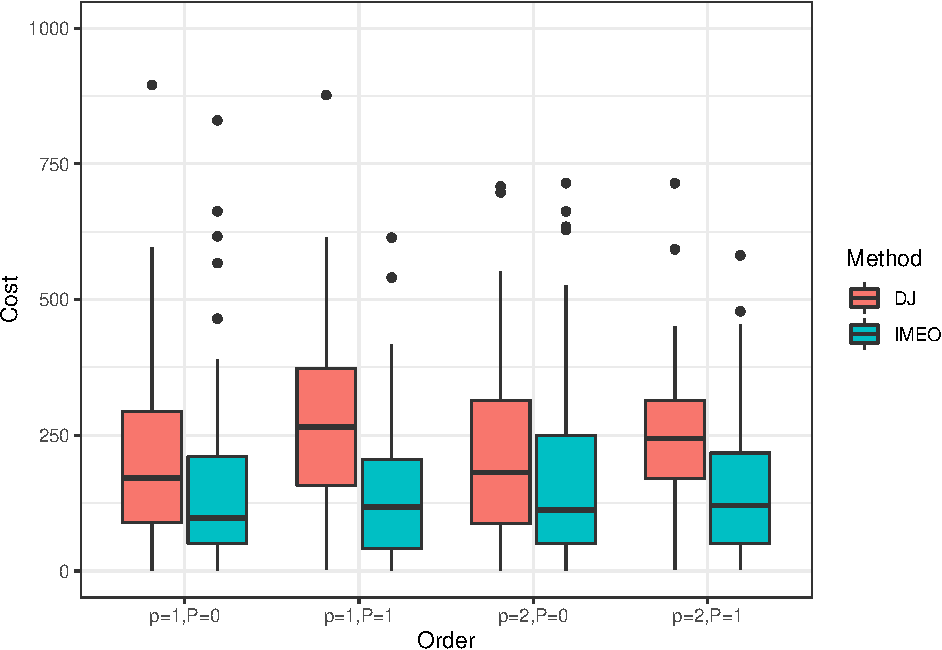
\includegraphics{Real_files/figure-latex/boxplot-1.pdf}

\begin{Shaded}
\begin{Highlighting}[]
\KeywordTok{ggplot}\NormalTok{(df, }\KeywordTok{aes}\NormalTok{(}\DataTypeTok{x=}\NormalTok{lag_length, }\DataTypeTok{y=}\NormalTok{error_record, }\DataTypeTok{fill=}\NormalTok{Method)) }\OperatorTok{+}
\StringTok{  }\KeywordTok{coord_cartesian}\NormalTok{(}\DataTypeTok{ylim =} \KeywordTok{c}\NormalTok{(}\OperatorTok{-}\DecValTok{100}\NormalTok{, }\DecValTok{100}\NormalTok{)) }\OperatorTok{+}
\StringTok{  }\KeywordTok{geom_boxplot}\NormalTok{(}\KeywordTok{aes}\NormalTok{(}\DataTypeTok{middle =} \KeywordTok{mean}\NormalTok{(error_record))) }\OperatorTok{+}\StringTok{ }\KeywordTok{theme_bw}\NormalTok{() }\OperatorTok{+}\StringTok{ }
\StringTok{  }\KeywordTok{labs}\NormalTok{(}\DataTypeTok{x =} \StringTok{"Order"}\NormalTok{, }\DataTypeTok{y =}  \StringTok{"Error"}\NormalTok{)}
\end{Highlighting}
\end{Shaded}

\includegraphics{Real_files/figure-latex/boxplot-2.pdf}

\end{document}
